\chapter{MisMatchFinder - supplementary methods}
\label{ch-mmfSuppMeth}

\section{ROI bed files generation}
\label{ch-mmfAppendix:bedfiles}

To ensure optimal mapping rates and no mapping related mismatches, the analysis is restricted to high mappability areas of the genome. These areas were defined as regions, where a k-mer of 100bp has a 85\% or higher unique mappability rate. The mappability tracks were first computed with GEM \cite{Derrien2012} and then collated converted to a bed file with R just like in the best practice instructions of QDNAseq \cite{Scheinin2014} for creating a new bin annotation. This method is only required for GRCh38 \cite{Schneider2017} as so far, the UCSC data track is only available for GRCh37 \cite{Church2011}.

\section{Oligo-nucleotide context normalisation}
\label{ch-mmfAppendix:oligoNorm}
The ROI restriction of the analysis from \autoref{ch-mmfAppendix:bedfiles} automatically leads to a different tri- and di-nucleotide context frequency in the analysed regions, than the rest of the genome, which was used to generate the original signatures \cite{Alexandrov2020}. For this reason, MisMatchFinder analyses the oligo-nu\-cle\-o\-tide composition of the analysed regions and generates weighted counts by adjusting for the differences. 

The baseline frequencies of both di- and tri-nucleotides were generated with the function \textit{oligonucleotideFrequency} from the ``Biostrings`` library \cite{Pages2020} using the hg38 BSgenome \cite{Pages2020a}. The raw counts of the di- and tri-nucleotides can be seen in \autoref{A:mmf:tab:dicounts} and \autoref{A:mmf:tab:tricounts} respectively.





\begin{table}[!ht]
\caption[Dinucleotide counts of GRCh38]{Dinucleotide counts generated with Biostrings \cite{Pages2020} for GRCh38}\label{A:mmf:tab:dicounts}
\centering
\rowcolors{2}{gray!15}{white}
\begin{tabular}{|C{0.2\linewidth} | R{0.2\textwidth}|}
\toprule
 \hline
 \rowcolor{gray!50}
 \textbf{DINUCLEOTIDE} & \textbf{COUNT}\\
 \hline
       AA   & \num{287025139} \\
       AC   & \num{148150331} \\
       AG   & \num{205752406} \\
       AT   & \num{226225785} \\
       CA   & \num{212880749} \\
       CC   & \num{151236932} \\
       CG   & \num{29401795} \\
       CT   & \num{205524144} \\
       GA   & \num{175847498} \\
       GC   & \num{124732844} \\
       GG   & \num{152432158} \\
       GT   & \num{148502457} \\
       TA   & \num{191400248} \\
       TC   & \num{174923630} \\
       TG   & \num{213928532} \\
       TT   & \num{289690054} \\ 
 \hline
 \bottomrule
\end{tabular}
\end{table}

\begin{table}[!ht]
\caption[Trinucleotide counts of GRCh38]{Trinucleotide counts generated with Biostrings \cite{Pages2020} for GRCh38}\label{A:mmf:tab:tricounts}
\centering
\rowcolors{2}{gray!15}{white}
\begin{tabular}{|C{0.2\linewidth} | R{0.15\linewidth}| C{0.04\linewidth} |C{0.2\linewidth} | R{0.15\linewidth}|}
\toprule
 \hhline{|-|-|~|-|-|}
 \rowcolor{gray!50}
 \textbf{TRINUCLEOTIDE} & \textbf{COUNT} & \cellcolor{white} & \textbf{TRINUCLEOTIDE} & \textbf{COUNT}\\
 \hhline{|-|-|~|-|-|}

AAA & \num{ 112465943} & \cellcolor{white} & GAA & \num{ 58990420} \\
AAC & \num{ 43532050} & \cellcolor{white} & GAC & \num{ 27737004} \\
AAG & \num{ 58439928} & \cellcolor{white} & GAG & \num{ 49560877} \\
AAT & \num{ 72587151} & \cellcolor{white} & GAT & \num{ 39559024} \\
ACA & \num{ 59305516} & \cellcolor{white} & GCA & \num{ 42481943} \\
ACC & \num{ 33784390} & \cellcolor{white} & GCC & \num{ 34497599} \\
ACG & \num{ 7584302} & \cellcolor{white} & GCG & \num{ 7078395} \\
ACT & \num{ 47476086} & \cellcolor{white} & GCT & \num{ 40674873} \\
AGA & \num{ 65552680} & \cellcolor{white} & GGA & \num{ 46022042} \\
AGC & \num{ 41073623} & \cellcolor{white} &GGC & \num{ 34474720} \\
AGG & \num{ 51723263} & \cellcolor{white} &GGG & \num{ 38148838} \\
AGT & \num{ 47402783} & \cellcolor{white} &GGT & \num{ 33786518} \\
ATA & \num{ 60308591} & \cellcolor{white} &GTA & \num{ 33265786} \\
ATC & \num{ 39076747} & \cellcolor{white} &GTC & \num{ 27466578} \\
ATG & \num{ 53548035} & \cellcolor{white} &GTG & \num{ 44578403} \\
ATT & \num{ 73292370} & \cellcolor{white} &GTT & \num{ 43191653} \\
CAA & \num{ 55220609} & \cellcolor{white} &TAA & \num{ 60348082} \\
CAC & \num{ 44001434} & \cellcolor{white} &TAC & \num{ 32879810} \\
CAG & \num{ 59791771} & \cellcolor{white} &TAG & \num{ 37959659} \\
CAT & \num{ 53866888} & \cellcolor{white} &TAT & \num{ 60212654} \\
CCA & \num{ 53293160} & \cellcolor{white} &TCA & \num{ 57800075} \\
CCC & \num{ 38036593} & \cellcolor{white} &TCC & \num{ 44918305} \\
CCG & \num{ 8026845} & \cellcolor{white} &TCG & \num{ 6712244} \\
CCT & \num{ 51880303} & \cellcolor{white} &TCT & \num{ 65492835} \\
CGA & \num{ 6511692} & \cellcolor{white} &TGA & \num{ 57760931} \\
CGC & \num{ 7021552} & \cellcolor{white} &TGC & \num{ 42162935} \\
CGG & \num{ 8229568} & \cellcolor{white} &TGG & \num{ 54330453} \\
CGT & \num{ 7638969} & \cellcolor{white} &TGT & \num{ 59674158} \\
CTA & \num{ 37666053} & \cellcolor{white} &TTA & \num{ 60159779} \\
CTC & \num{ 49481013} & \cellcolor{white} &TTC & \num{ 58899235} \\
CTG & \num{ 59039769} & \cellcolor{white} &TTG & \num{ 56762262} \\
CTT & \num{ 59337262} & \cellcolor{white} &TTT & \num{ 113868707} \\
\hhline{|-|-|~|-|-|}
\bottomrule
\end{tabular}
\end{table}

\afterpage{\clearpage}


\section{Germline filtering with zarr}
\label{ch-mmfAppendix:germlineFilter}
As shown in \autoref{fig:mmf-mismatchrate}A, the amount of mismatches found in a 10x coverage sample can easily exceed $3$ million. In addition to that, the current gnomAD database contains $ \approx 707$ million variants. This means a normal merge for two datasets based on chromosomal position is not feasible for a normal compute resource in a acceptable time frame. To allow an easy query of mismatch positions against the full database, a zarr \cite{Miles2021}representation of the gnomAD VCF was generated. However in contrast to the out of the box indexing function shipped with skikit-allel \cite{Miles2021a} which was used to convert the vcf to zarr, the program uses its own index built with ncls, which is available through PyRanges \cite{Stovner2019}. The sections below outline first the conversion process with scikit-allel (\autoref{ch-mmfAppendix:zarr}) and then details the filtering in the MisMatchFinder program (\autoref{ch-mmfAppendix:filter})

\subsection{Zarr conversion with scikit-allel}
\label{ch-mmfAppendix:zarr}
While it is easy to access a zarr archive, both for reading and writing, once it is created, the generation requires time. The time is mostly computational and not so much development, as the scikit-allel package contains the function \lq\emph{allel.vcf\_to\_zarr}\rq, which allows the direct conversion of VCF to zarr with only a few prerequisites. 

Importantly, tabix \cite{Li2011} can be used to split the conversion into multiple parts by restricting the process to specific regions.

\autoref{lst-mmfAppendix:zarr} shows the code used to convert chromosome \lq chr1 \rq from the downloaded gnomad vcf

\begin{lstlisting}[language=Python, caption=scikit-allel conversion vcf\_to\_zarr, label={lst-mmfAppendix:zarr}]
import scikit-allel as allel

allel.vcf_to_zarr(input="gnomad.genomes.r3.1.2.sites.vcf.bgz", output="/out/put/folder/",  group="chr1", region="chr1", fields="*")
\end{lstlisting}

When MisMatchFinder is installed on your system, the function \lq\emph{generateZarrStorage}\rq\ is a wrapper, which allows the parallel conversion as well to resume a failed or incomplete attempt. It is equivalent to the above code and has only usability and ease of access as priorities. This automated version will convert all fields, which include fields never used in MisMatchFinder to optimise the memory footprint of the zarr representation, the option fields in \autoref{lst-mmfAppendix:zarr} can be set to the value shown in \autoref{lst-mmfAppendix:fields}.
\begin{lstlisting}[language=Python, caption=field options for reduced memory, label={lst-mmfAppendix:fields}]
fields="['variants/CHROM', 'variants/POS', 'variants/REF', 'variants/ALT', 'variants/AF', 'variants/FILTER_PASS']"
\end{lstlisting}
Which contains only the information used in MisMatchFinder. The same result can be achieved with adding the option \lq --$mandatoryOnly$ \rq to the supplied wrapper.

\todo[inline, color=red]{actually implement the wrapper i am talking about here}

\subsection{MisMatchFinder filtering - the zarr API}
\label{ch-mmfAppendix:filter}

\subsection{Data simulation}
\label{ch-mmfAppendix:simulation}
This section contains all the additional information required to replicate the simulation of data used in the MisMatchFinder chapter (\autoref{ch:mmf})

\subsection{Signature simulation - we can spike this punch}
\label{ch-mmfAppendix:spikein}
This section describes the signature spike-in simulation. The full code of the variant selection is available in \autoref{lst-mmfAppendix:spikeInSelect} with the bamsurgeon code shown in \autoref{lst-mmfAppendix:spikeInMut}.

For the selection of variants to spike-in with bamsurgeon, I use the fully annotated ``CosmicMutantExport.tsv`` from \href{https://cancer.sanger.ac.uk/cosmic/download}{\nolinkurl{https://cancer.sanger.ac.uk/cosmic/download}}, then restrict the list to SNPs. These are loaded into R and annotated with their tri-nucleotide context. Because the signatures are based on the pyrimidine nucleotides, the reverse complement is generated for variants with a purine in the center position.

The sampling amount is calculated by using the intended signatures percentages (e.g. \autoref{fig:sig7a}, \autoref{A:fig:sig3}) and multiplying with the desired amount of variants, which can be derived from the chosen mutation rate in per million (\autoref{A:eq:desiredVars}).

\begin{equation}
n(variants) = \frac{mutation~rate}{1\cdot10^{6} \cdot genome~length}
\label{A:eq:desiredVars}
\end{equation}

For our data, we assume a genome length of $3 \cdot 10^9$ and use four different mutations rates (0.1, 5, 25, 50 and 100). For the final sampling I used ``data.table`` and finally variants are assign an allele frequency of 0.1.


\begin{lstlisting}[language=R, caption=spike-in variant selection, label={lst-mmfAppendix:spikeInSelect}]
#get the snps
bed <- data.table(read.table("/data/reference/dawson_labs/COSMIC/v92/CosmicMutantSNPs.bed", sep="\t"))
colnames(bed) <- c("chr", "start", "end", "ref", "alt", "cancer", "status")

#get the surrounding variants
varTriNuc <- GRanges(seqnames=bed$chr, IRanges(start=(bed$start-1), end=(bed$end+1)))

#select the right genome
genome <- BSgenome.Hsapiens.UCSC.hg38::BSgenome.Hsapiens.UCSC.hg38

#get trinucs
seq <- Biostrings::getSeq(genome, varTriNuc)

# if we dont have a C or a T as the ref, we build the reverse complement, because thats
# what the signatures are based on
seq[bed$ref %in% c("G", "A")] <- Biostrings::reverseComplement(seq[bed$ref %in% c("G", "A")])

#put the trinucs with the variants
bed[,tri:= as.character(seq) ]
#add in the trinuc alt, so that we know where things are goings
bed[,triAlt:=ifelse(ref %in% c("C", "T"), alt, as.character(Biostrings::complement(Biostrings::DNAStringSet(bed$alt))))]

#now we build the name of the trinuc change as it is used in COSMIC
bed[,cosmicName:=paste(tri,triAlt)]
bed[,cosmicName:=gsub(pattern="(.)(.)(.) (.)", replacement = "\\1[\\2>\\4]\\3", cosmicName)]

#read in the signatures profile
sig7a <- data.table(read.table("/home/shollizeck/workspace/myDawsonRep/TMB/v3.2_SBS7a_PROFILE.txt", header=T, sep="\t"))

# mutations per megabase
rate <- 100

nVars <- rate/1E6*3E9

#get the number of each trinucChange we need
numCols <- colnames(sig7a)[-1]
sig7a[,(numCols):=lapply(.SD, function(x) round(x*nVars)), .SDcols=numCols]

#merge the two tables together to enable sampling
sampleTableSBS7a <- merge(bed, sig7a, by.x="cosmicName", by.y="X")

selectionSBS7a <- sampleTableSBS7a[,.SD[sample(.N,size=SBS7a_GRCh38)], by="cosmicName"]

#add in the frequency (VAF) of the variants which is a uniform 10%
selectionSBS7a[,vaf:=0.1]
\end{lstlisting}

With the generated bed, bamsurgeon can be used to create the final mutated BAM. As we are using low coverage WGS as input, some parameters need to be adjusted to allow variants to be generated. Mostly, we need to allow bamsurgeon to even mutate regions with very low coverage (\lq\emph{--mindepth~1}\rq), ignore the pileup of the original (\lq\emph{--ignorepileup}\rq), allow a higher coverage difference (\lq\emph{-d~0.7}\rq) and lastly allow bamsurgeon to NOT mutate a position (\lq\emph{--minmutreads~0}\rq). To make the data creation reproducible, we also assign a seed of 1234.

After the BAM generation, the actually spiked-in variants are generated sorted and indexed.

Lastly, the bam needs to be postprocessed to be in line with the SAM specifications (\autoref{lst-mmfAppendix:spikeInMut}).

\begin{lstlisting}[language=bash, caption=bamsurgeon spike-in, label={lst-mmfAppendix:spikeInMut}]
bamsurgeon addsnv.py -d 0.7 --ignorepileup --mindepth 1 --minmutreads 0 -v mutations.bed -r $reference -o mutated.bam --aligner mem --seed 1234 -f input.bam

bamsurgeon makevcf.py addsnv_logs_mutated.bam | vcfstreamsort -a | bcftools view -o variants.vcf.gz -O z && bcftools index -t variants.vcf.gz

bamsurgeon  postprocess.py -f ${reference}.fai mutated.bam
\end{lstlisting}


\subsection{Patient data subsampling}
\label{ch-mmfAppendix:subsampling}
Subsampling of high depth WGS data was done with samtools (v1.13) supplying random seeds, but stable sampling rates. Sampling rates were selected, such that the output file would have an average coverage of 10x to be comparable with other sequencing data.


\chapter*{Supplementary Figures}

\begin{figure}[!ht]
\centering
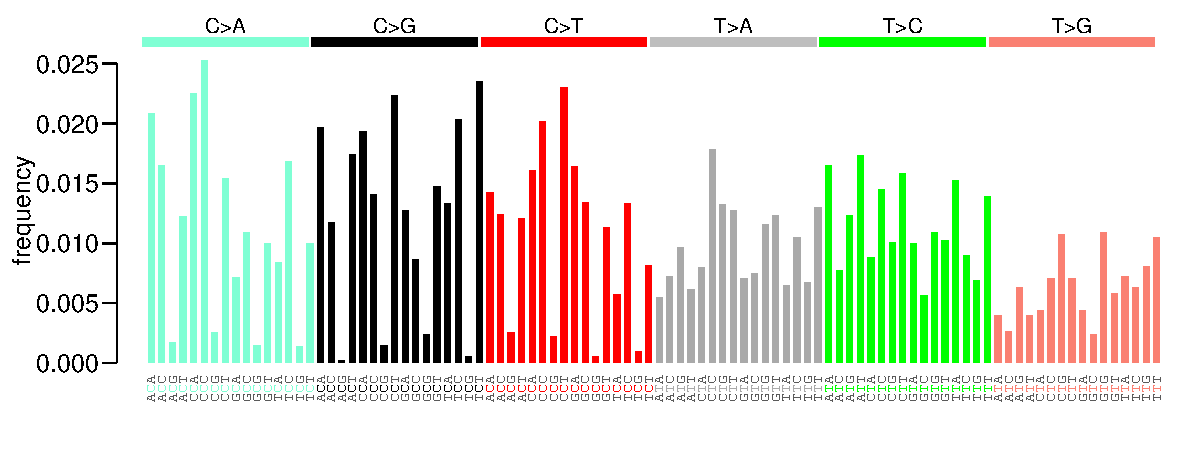
\includegraphics[width=.99\linewidth]{Figures/MisMatchFinder/SBS3Signature.pdf}
\caption[Trinculeotide count contributions for single base substitution (SBS) signature 3]{Trinculeotide count contributions for SBS signature 3 (Defective homologous recombination-based DNA damage repair); values taken from \protect\textcite{Alexandrov2020}}\label{A:fig:sig3}
\end{figure}

\begin{figure}[!ht]
\centering
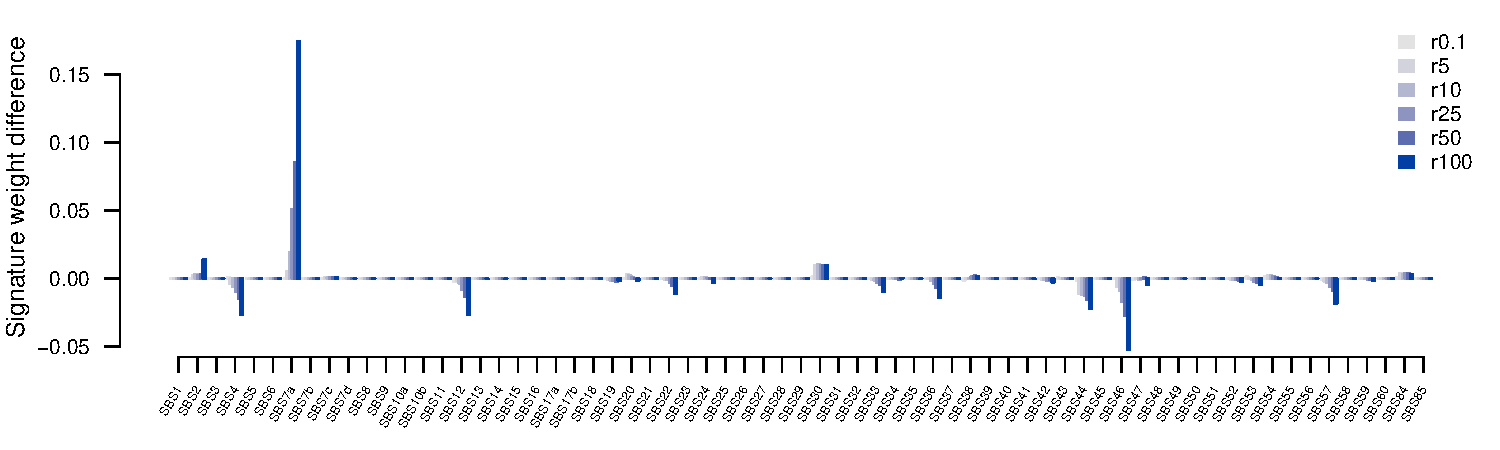
\includegraphics[width=.99\linewidth]{Figures/MisMatchFinder/SBS7SpikeInSignatureDifferences.pdf}
\caption[Signature weights differences from normal for SBS7a spike-in]{Signature weights differences from normal for SBS7a spike-in; Weights were deconstructed with QP method in MisMatchFinder and the weights assigned to the normal sample used for the spike-in were substracted; r0.1 corresponds to 0.1 mutations per megabase (287 variants) and r100 is the equivalent of 100 mutations per megabase (286974 variants)}\label{A:fig:sbs7aspikeindifferences}
\end{figure}

\begin{figure}[!ht]
\centering
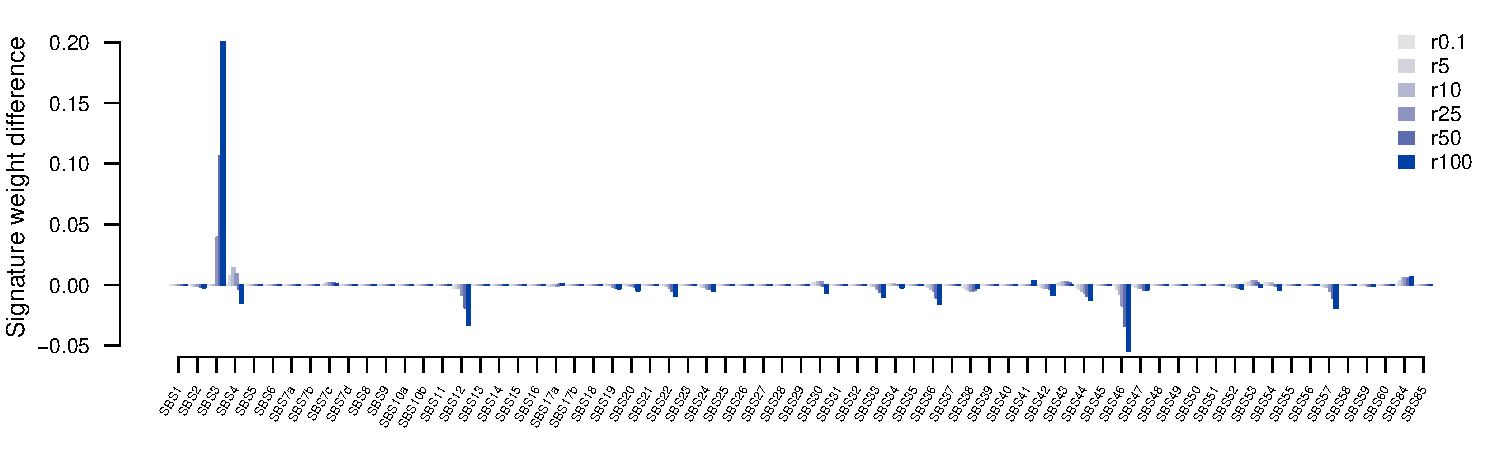
\includegraphics[width=.99\linewidth]{Figures/MisMatchFinder/SBS3SpikeInSignatureDifferences.pdf}
\caption[Signature weights differences from normal for SBS3 spike-in]{Signature weights differences from normal for SBS3 spike-in; Weights were deconstructed with QP method in MisMatchFinder and the weights assigned to the normal sample used for the spike-in were substracted; r0.1 corresponds to 0.1 mutations per megabase (264 variants) and r100 is the equivalent of 100 mutations per megabase (285367 variants)}\label{A:fig:sbs3spikeindifferences}
\end{figure}

\begin{figure}[!ht]
\centering
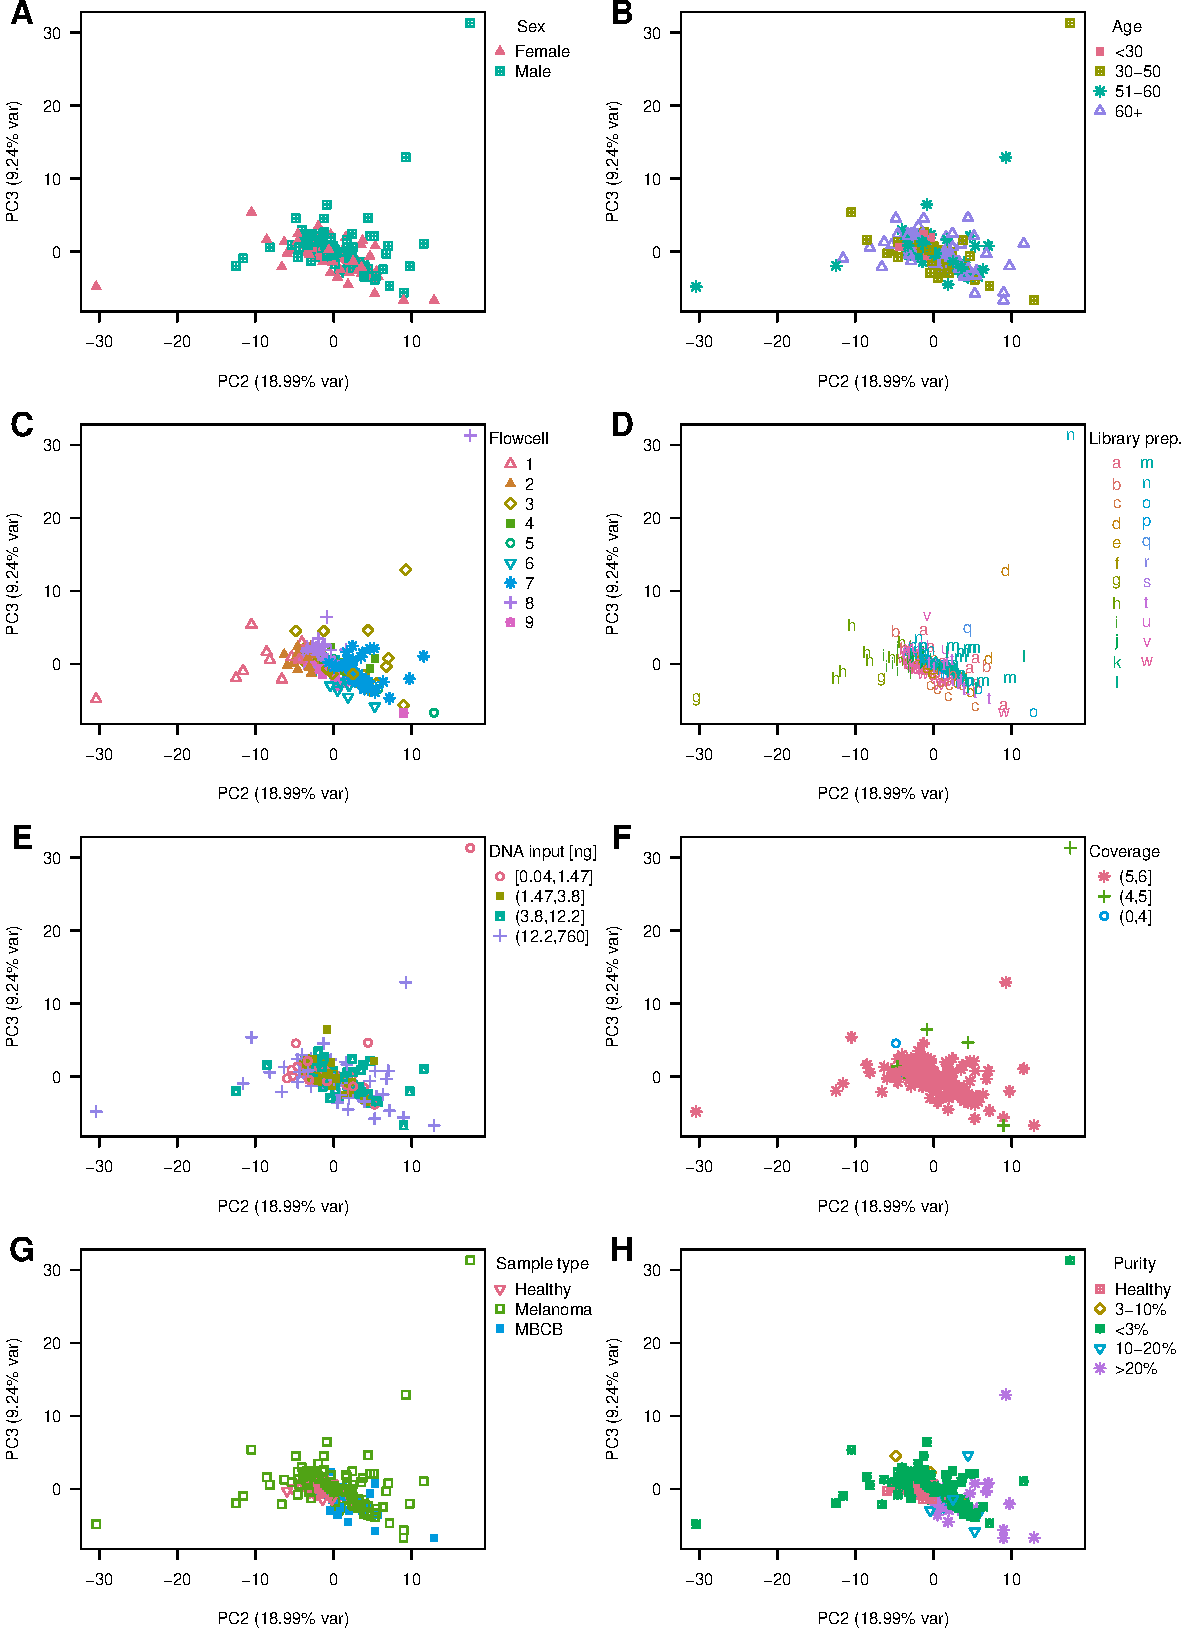
\includegraphics[width=.99\linewidth]{Figures/MisMatchFinder/countPCAsPC2vsPC3.pdf}
\caption[PCA of tri-nucleotide mismatch counts of real world data (PC2 and PC3)]{PCA (PC2 and PC3) of tri-nucleotide mismatch counts of healthy donor and tumour samples (melanoma and metastatic breast cancer) of varying purity; PCA was conducted on scaled and centered data}\label{A:fig:mmf-pca2v3}
\end{figure}

